\documentclass[titlepage]{jarticle}
\usepackage{h31ec-exp}
\usepackage[dvipdfmx]{graphicx}
\usepackage[yen]{okuverb}
\usepackage{here}

\title{題名をかいてね}
\grade{3年40番}%
\author{鷲尾 優作}
\team{}
\date{令和2年7月8日}
\expdate{令和2年7月13日}
\coauthor{
  %26番 & 滝沢 倖大\\
  %31番 & 原山 蓮\\
  %34番 & 西脇 光
}

\begin{document}
\maketitle

\section{本実験の目的}
\begin{itemize}
    \item なんちゃらかんちゃら
\end{itemize}

\section{理論}
直列回路の場合の負荷で消費される電力P[W]は、電圧V[V]、電流I[A]として、$P=V・I$と計算できる。
一方、交流回路の場合、負荷で消費される電力P[W]は、電圧V[V]、電流I[A]、電圧と電流の位相差$Φ$として式(1)で計算される\\

\begin{equation}
    P=V・I・cos(Φ)
\end{equation}
この電力のことを有効電力と呼ぶ。一般の電力計はこの有効電力を測定するものである。有効電力を単に電力と呼ぶ場合が多い。
式(1)中の$cos(Φ)$は、電圧と電流の積$(V・I)$のうち、有効電力として消費される割合を示すものであり、力率と呼ばれる。また、電圧と電流の積$(V・I)$は、実際に負荷で消費される電力ではなく、見かけの電力であり、皮相電力と呼ばれる。単位は[VA]が用いられる。\\
まとめると次のようになる.\\
\begin{equation}
    皮相電力	 Ps=V・I	        [VA]
\end{equation}
\begin{equation}
    有効電力(電力)   P=V・I・cos(Φ)   [W]
\end{equation}
\begin{equation}
    無効電力     Q=V・I・sin(Φ)    [var]
\end{equation}
\begin{equation}
    力率		 cos(Φ)=P/Ps
\end{equation}

\section{実験内容}
負荷として白熱電球を用い、その皮相電力、有効電力(電力)、力率を測定する。また、負荷にコンデンサを追加し、同様の測定を行い力率等の変化を調べる。
第1図において、電力計は負荷の有効電力を測定する測定器である。電圧計・電流計で電圧値V、電流値Iを測定し、皮相電力Psを求める。有効電力Pは電力計で測定されるから、力率は式(5)で求めることができる。

\section{使用器具}
\begin{enumerate}
    \item スライダック\\用途 交流電源確保のため\\商品名TYPE S-130-10\\物品番号B27 1 43
    \item 交流電圧計\\用途 交流電圧計測のため\\商品名YOKOGAWA\\物品番号L119 1 184
    \item 交流電流計\\用途 交流電流計測のため\\商品名YOKOGAWA\\物品番号L116 1 225
    \item 電力計\\用途 実験データ計測のため\\商品名YOKOGAWA\\物品番号L142 1 81
    \item 白熱電球負荷\\用途 実験用負荷\\商品名National 110V60W\\物品番号なし
    \item コンデンサ\\用途 実験データ計測のため\\商品名National N2形 SH(MF) No.5\\物品番号なし
\end{enumerate}

\section{測定}
\subsection{白熱電球負荷の測定}
\begin{figure}[H]
    \begin{center}
        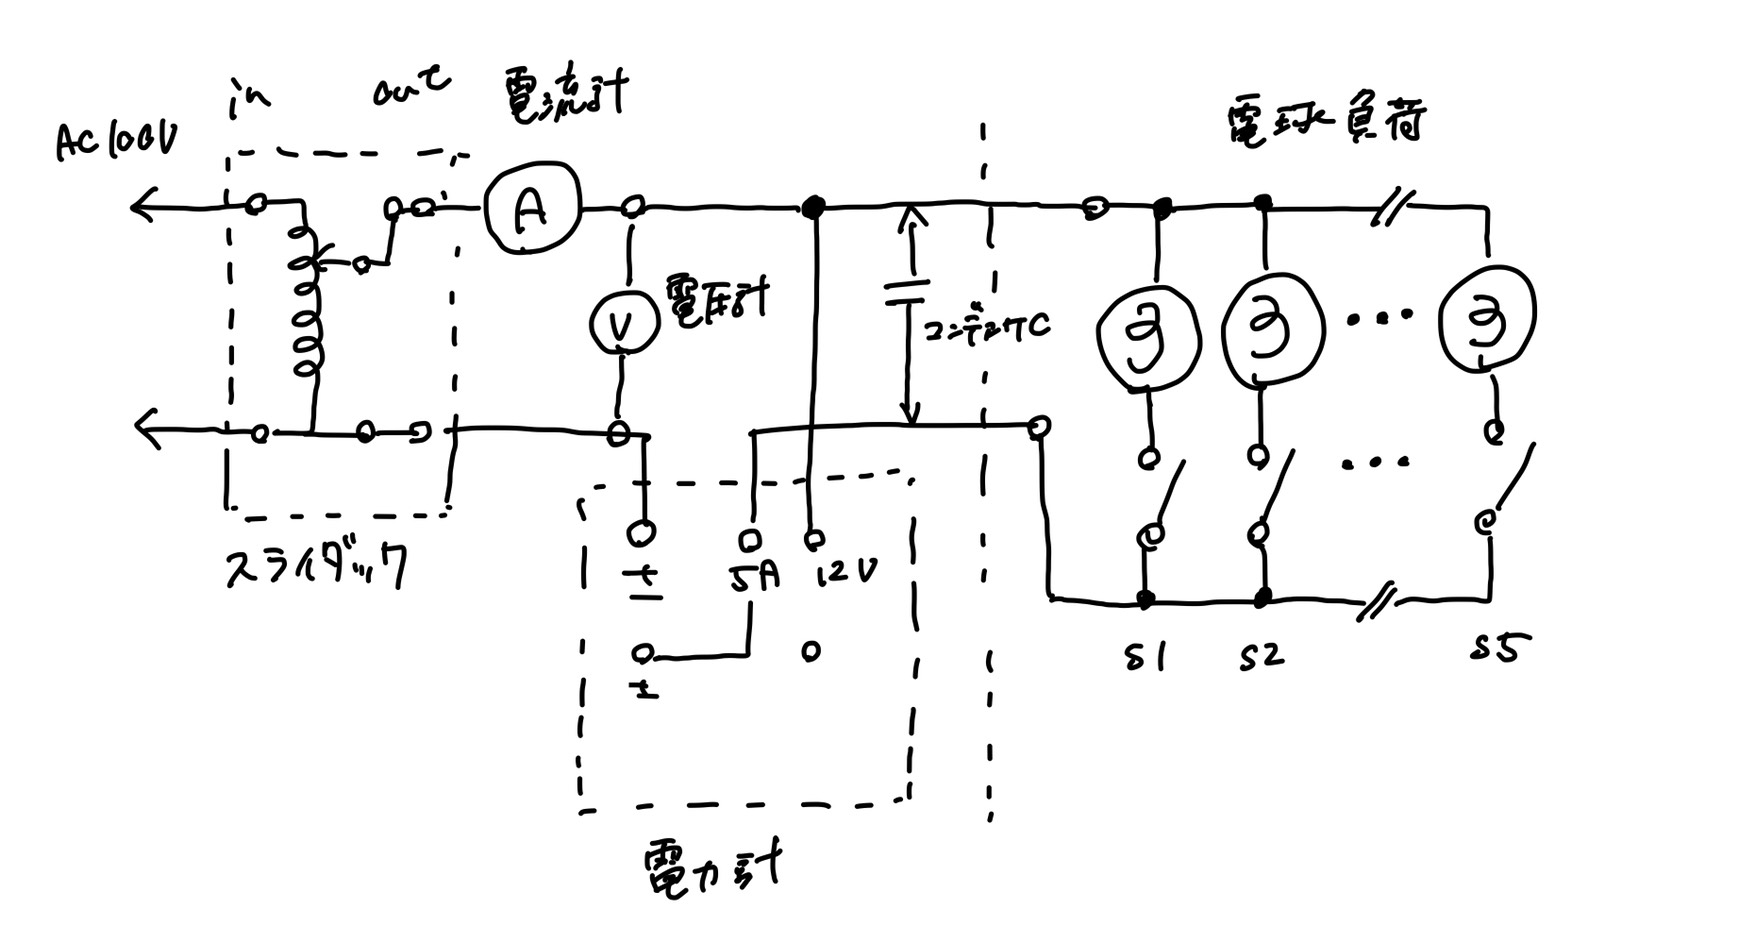
\includegraphics[width=10cm]{image/1.jpg}
        \caption{電力測定接続図}
    \end{center}
\end{figure}
\begin{enumerate}
    \item 図1のように接続する。コンデンサは接続しない
    \item 負荷のスイッチS1をONとし、スライダックを調節、電圧値を100Vに設定する。
    \item 電流、電圧値を測定する。
    \item 電圧値を100[V]に一定に保ちながら、負荷スイッチS2→S5をONにし、その都度電流、電力値を測定する。
\end{enumerate}


\subsection{白熱電球負荷にコンデンサを追加した場合の測定}
コンデンサを接続し、3.1.1と同様の測定をする。\\
コンデンサの容量は50、100[μF]の2種類。

\section{測定結果}


\begin{table}[htbp]
    \caption{}
    \begin{tabular}{l|r|r|r|r|r|r|r}
        \multicolumn{ 8}{c}{白熱電球負荷}                                                                                                                                                                                                                                \\ \hline
        \multicolumn{ 1}{c|}{負荷スイッチ} & \multicolumn{ 1}{c|}{電圧V[V]} & \multicolumn{ 1}{c|}{電流I[A]} & \multicolumn{ 1}{c|}{皮相電力Ps[VA]} & \multicolumn{ 3}{c|}{電力[W]} & \multicolumn{ 1}{c}{力率[\%]}                                                      \\ \cline{ 5- 7}
        \multicolumn{ 1}{l|}{}             & \multicolumn{ 1}{l|}{}         & \multicolumn{ 1}{l|}{}         & \multicolumn{ 1}{l|}{}               & \multicolumn{1}{l|}{ふれ}     & \multicolumn{1}{l|}{定数}     & \multicolumn{1}{l|}{電力P} & \multicolumn{ 1}{l}{} \\ \hline \hline
        S1                                 & 100.0                          & 0.5                            & 52.0                                 & 11.0                          & 5                             & 55.0                       & 105.8                 \\ \hline
        S2                                 & 100.0                          & 1.1                            & 105.0                                & 21.0                          & 5                             & 105.0                      & 100.0                 \\ \hline
        S3                                 & 100.0                          & 1.6                            & 156.0                                & 31.0                          & 5                             & 155.0                      & 99.4                  \\ \hline
        S4                                 & 100.0                          & 2.1                            & 210.0                                & 42.0                          & 5                             & 210.0                      & 100.0                 \\ \hline
        S5                                 & 100.0                          & 2.6                            & 260.0                                & 52.5                          & 5                             & 262.5                      & 101.0                 \\ \hline
    \end{tabular}
    \label{}
\end{table}

\begin{table}[htbp]
    \caption{}
    \begin{tabular}{l|r|r|r|r|r|r|r}
        \multicolumn{ 8}{c}{白熱電球負荷・コンデンサ負荷 C=50[μF]}                                                                                                                                                                                                       \\ \hline
        \multicolumn{ 1}{c|}{負荷スイッチ} & \multicolumn{ 1}{c|}{電圧V[V]} & \multicolumn{ 1}{c|}{電流I[A]} & \multicolumn{ 1}{c|}{皮相電力Ps[VA]} & \multicolumn{ 3}{c|}{電力[W]} & \multicolumn{ 1}{c}{力率[\%]}                                                      \\ \cline{ 5- 7}
        \multicolumn{ 1}{c|}{}             & \multicolumn{ 1}{c|}{}         & \multicolumn{ 1}{c|}{}         & \multicolumn{ 1}{c|}{}               & \multicolumn{1}{l|}{ふれ}     & \multicolumn{1}{l|}{定数}     & \multicolumn{1}{l|}{電力P} & \multicolumn{ 1}{c}{} \\ \hline \hline
        S1                                 & 100.0                          & 1.8                            & 175.0                                & 11.0                          & 5                             & 55.0                       & 31.4                  \\ \hline
        S2                                 & 100.0                          & 2.0                            & 195.0                                & 21.0                          & 5                             & 105.0                      & 53.8                  \\ \hline
        S3                                 & 100.0                          & 2.3                            & 230.0                                & 32.0                          & 5                             & 160.0                      & 69.6                  \\ \hline
        S4                                 & 100.0                          & 2.7                            & 270.0                                & 42.5                          & 5                             & 212.5                      & 78.7                  \\ \hline
        S5                                 & 100.0                          & 3.1                            & 311.0                                & 52.5                          & 5                             & 262.5                      & 84.4                  \\ \hline
    \end{tabular}
    \label{}
\end{table}

\begin{table}[htbp]
    \caption{}
    \begin{tabular}{l|r|r|r|r|r|r|r}
        \multicolumn{ 8}{c}{白熱電球負荷・コンデンサ負荷 C=100[μF]}                                                                                                                                                                                                       \\ \hline
        \multicolumn{ 1}{c|}{負荷スイッチ} & \multicolumn{ 1}{c|}{電圧V[V]} & \multicolumn{ 1}{c|}{電流I[A]} & \multicolumn{ 1}{c|}{皮相電力Ps[VA]} & \multicolumn{ 3}{c|}{電力[W]} & \multicolumn{ 1}{c|}{力率[\%]}                                                      \\ \cline{ 5- 7}
        \multicolumn{ 1}{c|}{}             & \multicolumn{ 1}{c|}{}         & \multicolumn{ 1}{c|}{}         & \multicolumn{ 1}{c|}{}               & \multicolumn{1}{l|}{ふれ}     & \multicolumn{1}{l|}{定数}      & \multicolumn{1}{l|}{電力P} & \multicolumn{ 1}{c}{} \\ \hline \hline
        S1                                 & 100.0                          & 3.3                            & 328.0                                & 11.0                          & 5                              & 55.0                       & 16.8                  \\ \hline
        S2                                 & 100.0                          & 3.4                            & 339.0                                & 21.0                          & 5                              & 105.0                      & 31.0                  \\ \hline
        S3                                 & 100.0                          & 3.6                            & 360.0                                & 31.0                          & 5                              & 155.0                      & 43.1                  \\ \hline
        S4                                 & 100.0                          & 3.9                            & 385.0                                & 42.5                          & 5                              & 212.5                      & 55.2                  \\ \hline
        S5                                 & 100.0                          & 4.2                            & 416.0                                & 52.5                          & 5                              & 262.5                      & 63.1                  \\ \hline
    \end{tabular}
    \label{}
\end{table}
\newpage

\subsection{課題考察}
1)\\
固定インダクタに流れる電流の磁界と可動インダクタに流れる電流との間に生じる電流を使用して測定する.\\
2)\\
\begin{figure}[H]
    \begin{center}
        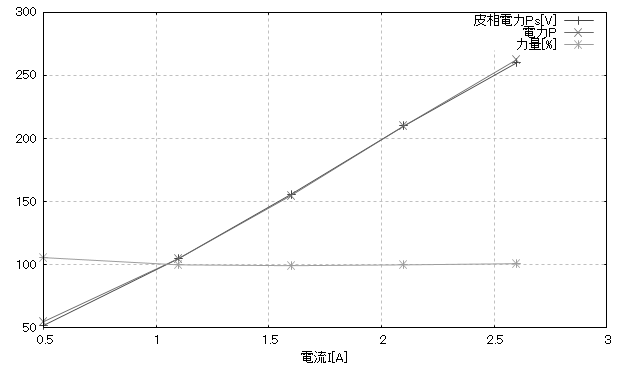
\includegraphics[width=15cm]{graph/g1.PNG}
    \end{center}
    \caption{特性グラフ}
\end{figure}

3)\\
エネルギーが低いため電圧降下が生じ効率が下がる\\
4)\\
コンデンサの容量性リアクタンス\\
一般家庭の電源用正弦波交流の角周波数は,$50×2×π = 100π$\\
よって,容量性リアクタンスは,C=50[μF]のとき\\
$1/5.0*10^-6*100π = 63.7$\\
C=100[μF]のとき\\
$1/1.0*10^-7*100π = 31.8$\\

コンデンサに流れる電流は,\\
I=V*2πfcなので,\\
C=50[μF]のとき22.1[A]\\
C=100[μF]のとき44.3[A]\\


\section{感想}
過去の実験で最も大電力を扱うものだったので安全に配慮して実験を行った,\\
交流回路での電力の表し方の方法にいくつかあり,必要に応じて使い分けなければならないことがわかった.

\end{document}